Il servizio GitHub fornisce un sistema per la gestione dei task e creazione di milestone.
Si è quindi deciso di utilizzare questo servizio.\\

\subsection{Creazione e gestione dei ticket}

I ticket vengono creati e gestiti quasi tutti dal responsabile di progetto.
Qualora il \textit{verificatore} trovasse imprecisioni o errori durante la verifica, avrà la possibilità di creare dei ticket per segnalare suddetti errori.
Ogni ticket può essere assegnato ad uno o più membri del gruppo a seconda della complessità del lavoro e della disponibilità dei membri del gruppo.
Per creare un nuovo ticket bisogna:

\begin{itemize}
	\item Andare su Issue;
	\item Premere "New issue";
	\item Compilare i campi richiesti:
		\begin{itemize}
			\item \textbf{Titolo e commenti:} titolo descrittivo con una descrizione del nuovo ticket;
			\item \textbf{Labels:} dovranno avere due caratteristiche fondamentali e cioè la tipologia di ticket assegnato(modifica, verifica, richiesta approvazione) e la priorità assegnata(alta, media, bassa);
			\item \textbf{Milestone:} la milestone a cui è associato il ticket;
			\item \textbf{Assignee:} a chi viene assegnato il ticket.
		\end{itemize}
\end{itemize}
\begin{figure}[h]
\centering
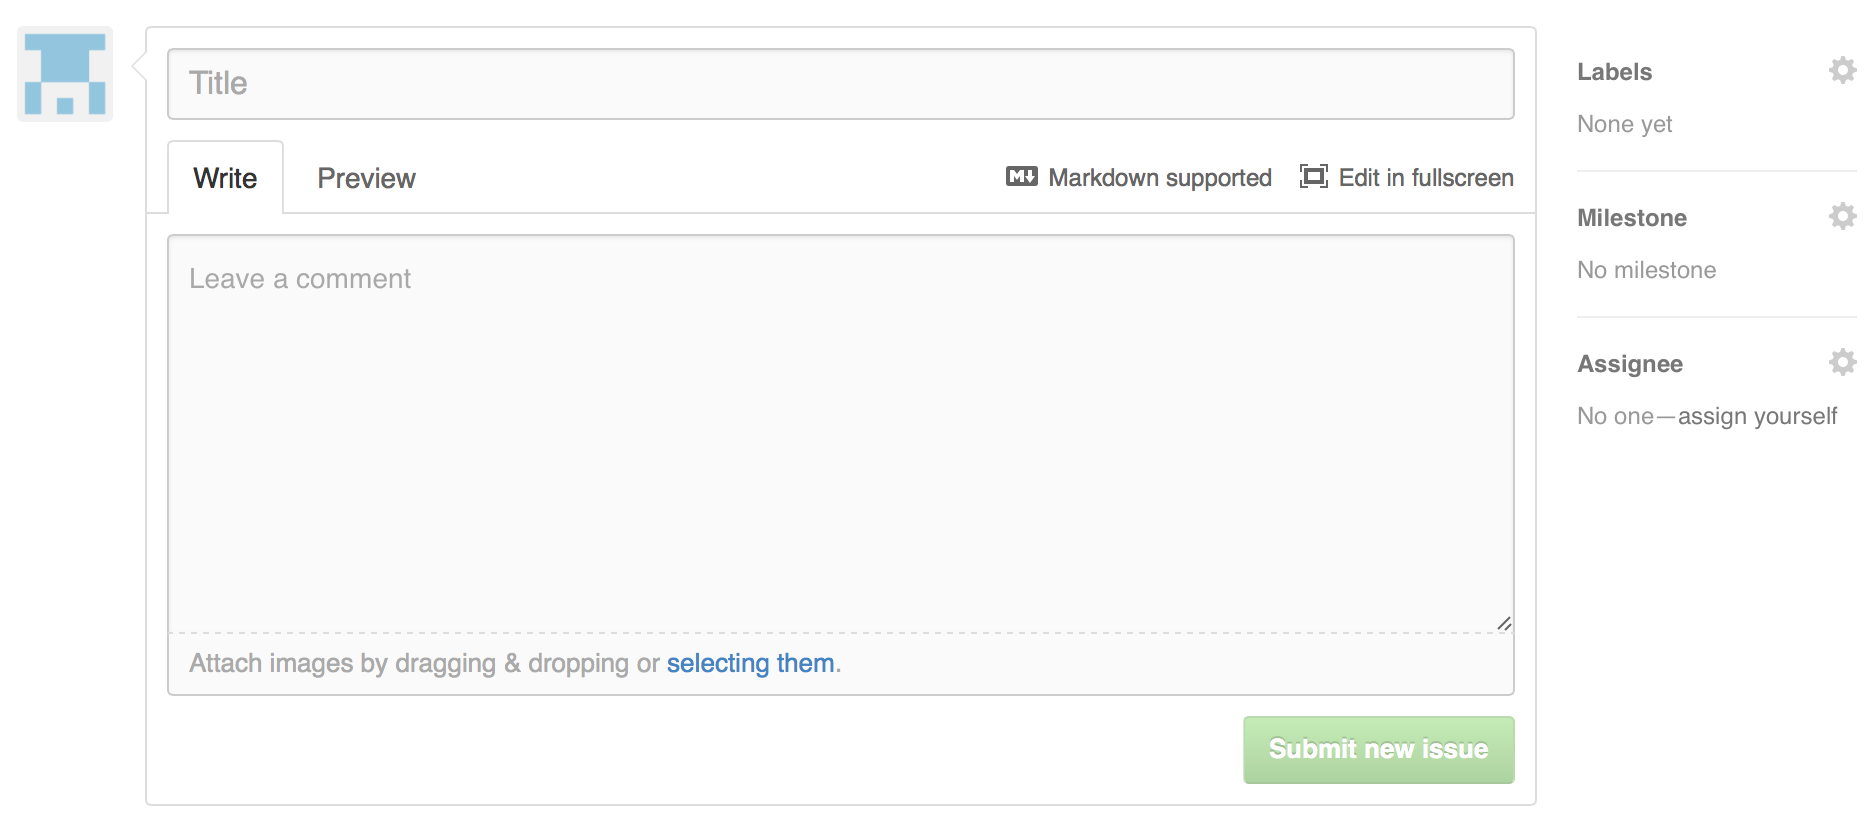
\includegraphics[width=0.7\linewidth]{img/ticket}
\caption[Creazione ticket]{Creazione ticket}
\label{fig:ticket}
\end{figure}


\subsection{Creazione delle milestone}

Il responsabile di progetto ha il compito della creazione di una milestone in occasione di ogni revisione al quale il gruppo \GRUPPO\ ha intenzione di partecipare, più altre milestone qualora il responsabile di progetto lo ritenga necessario.

Per creare una nuova milestone bisogna:

\begin{itemize}
	\item Andare su milestone;
	\item Premere "New milesone";
	\item Compilare i campi richiesti:
		\begin{itemize}
			\item \textbf{Titolo;}
			\item \textbf{Descrizione;}
			\item \textbf{Data.}
		\end{itemize}
\end{itemize}
\begin{figure}[h]
\centering
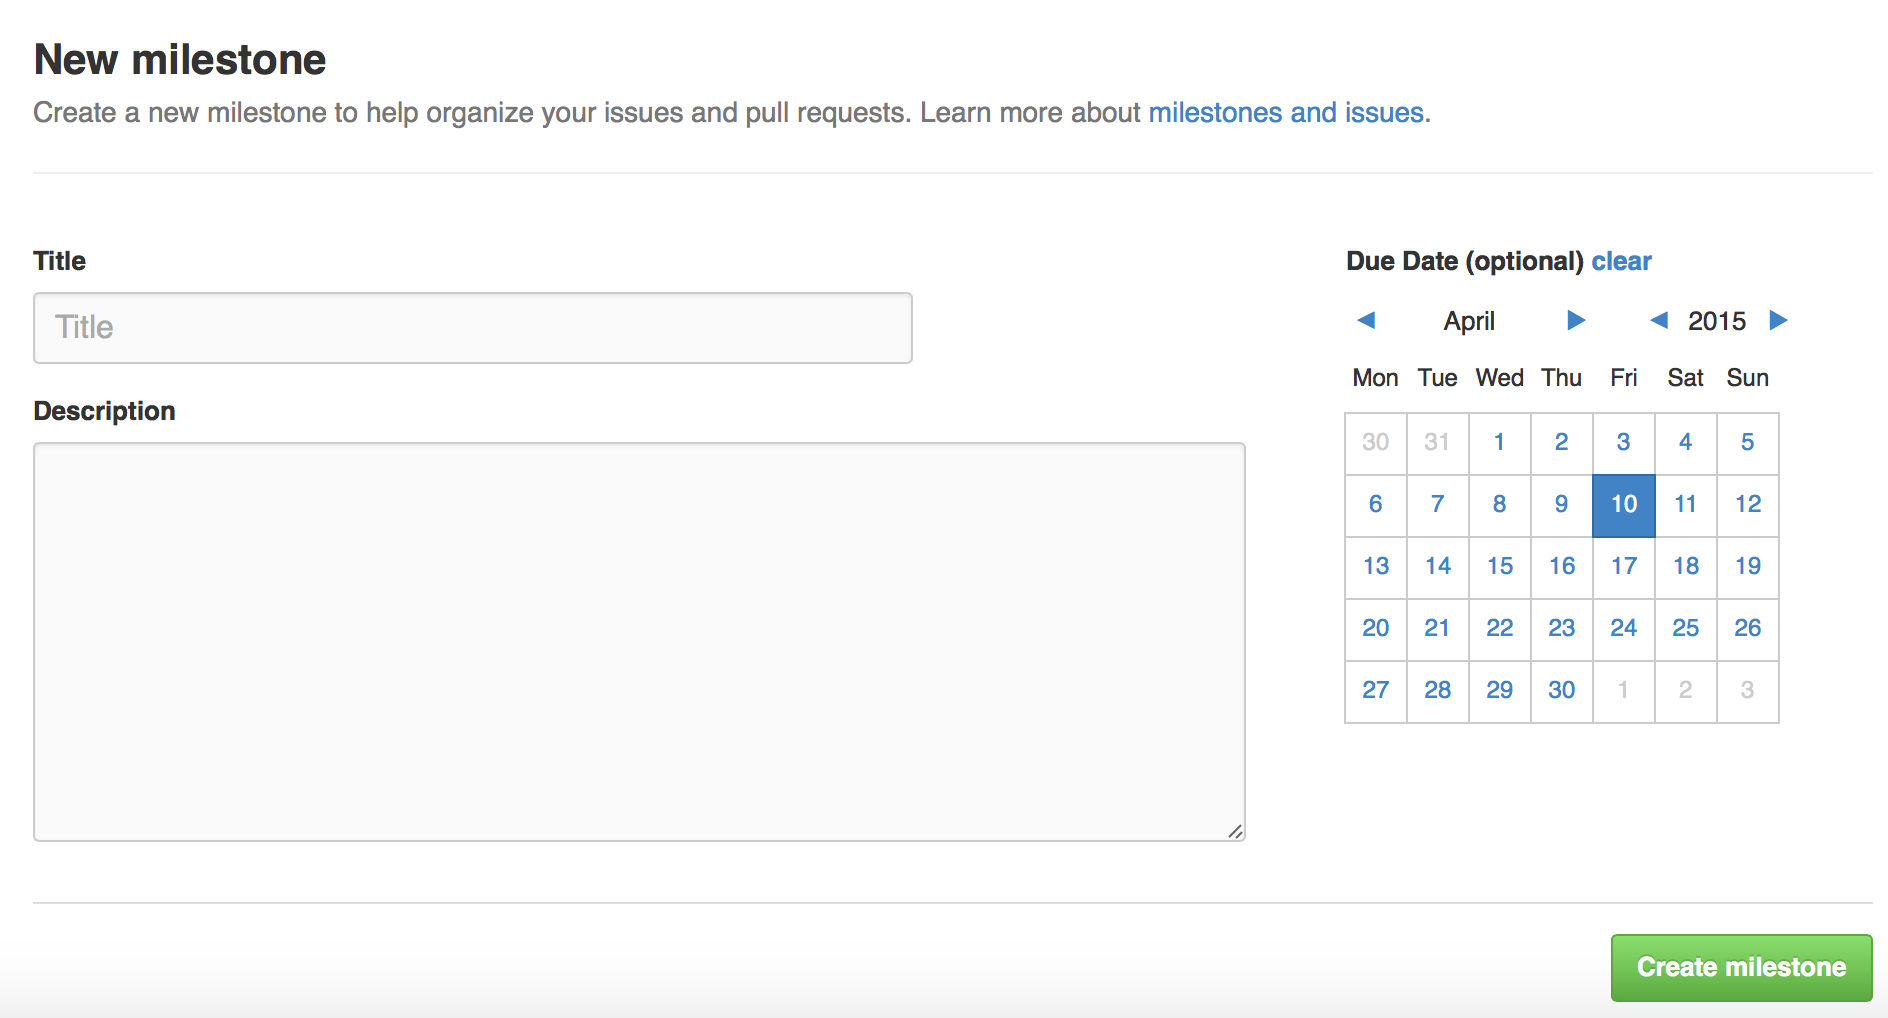
\includegraphics[width=0.7\linewidth]{img/milestone}
\caption[Creazione milestone]{Creazione milestone}
\label{fig:milestone}
\end{figure}


\subsection{Esecuzione dei compiti}

Ogni membro del gruppo è tenuto a visionare regolarmente la presenza di ticket a lui assegnati e segnalarne la presa in consegna.
Una volta che un membro porta a termine un ticket deve modificarne lo stato per segnalare il termine del lavoro.
Se un ticket non ha avuto i risultati attesi il \textit{Responsabile di Progetto} può riaprirlo ed eventualmente assegnare altri membri al lavoro.

\subsection{Chiusura della milestone}

Una volta raggiunta la scadenza, il \textit{Responsabile di Progetto}, deve chiudere la milestone ed eventualmente aprirne un'altra per poi ricominciare tutto il protocollo da capo.